\PassOptionsToPackage{unicode=true}{hyperref} % options for packages loaded elsewhere
\PassOptionsToPackage{hyphens}{url}
%
\documentclass[ignorenonframetext,]{beamer}
\usepackage{pgfpages}
\setbeamertemplate{caption}[numbered]
\setbeamertemplate{caption label separator}{: }
\setbeamercolor{caption name}{fg=normal text.fg}
\beamertemplatenavigationsymbolsempty
% Prevent slide breaks in the middle of a paragraph:
\widowpenalties 1 10000
\raggedbottom
\setbeamertemplate{part page}{
\centering
\begin{beamercolorbox}[sep=16pt,center]{part title}
  \usebeamerfont{part title}\insertpart\par
\end{beamercolorbox}
}
\setbeamertemplate{section page}{
\centering
\begin{beamercolorbox}[sep=12pt,center]{part title}
  \usebeamerfont{section title}\insertsection\par
\end{beamercolorbox}
}
\setbeamertemplate{subsection page}{
\centering
\begin{beamercolorbox}[sep=8pt,center]{part title}
  \usebeamerfont{subsection title}\insertsubsection\par
\end{beamercolorbox}
}
\AtBeginPart{
  \frame{\partpage}
}
\AtBeginSection{
  \ifbibliography
  \else
    \frame{\sectionpage}
  \fi
}
\AtBeginSubsection{
  \frame{\subsectionpage}
}
\usepackage{lmodern}
\usepackage{amssymb,amsmath}
\usepackage{ifxetex,ifluatex}
\usepackage{fixltx2e} % provides \textsubscript
\ifnum 0\ifxetex 1\fi\ifluatex 1\fi=0 % if pdftex
  \usepackage[T1]{fontenc}
  \usepackage[utf8]{inputenc}
  \usepackage{textcomp} % provides euro and other symbols
\else % if luatex or xelatex
  \usepackage{unicode-math}
  \defaultfontfeatures{Ligatures=TeX,Scale=MatchLowercase}
\fi
% use upquote if available, for straight quotes in verbatim environments
\IfFileExists{upquote.sty}{\usepackage{upquote}}{}
% use microtype if available
\IfFileExists{microtype.sty}{%
\usepackage[]{microtype}
\UseMicrotypeSet[protrusion]{basicmath} % disable protrusion for tt fonts
}{}
\IfFileExists{parskip.sty}{%
\usepackage{parskip}
}{% else
\setlength{\parindent}{0pt}
\setlength{\parskip}{6pt plus 2pt minus 1pt}
}
\usepackage{hyperref}
\hypersetup{
            pdftitle={Human Freedom Index},
            pdfauthor={Arpi Beshlikyan \& Jazmine Toledo},
            pdfborder={0 0 0},
            breaklinks=true}
\urlstyle{same}  % don't use monospace font for urls
\newif\ifbibliography
\usepackage{graphicx,grffile}
\makeatletter
\def\maxwidth{\ifdim\Gin@nat@width>\linewidth\linewidth\else\Gin@nat@width\fi}
\def\maxheight{\ifdim\Gin@nat@height>\textheight\textheight\else\Gin@nat@height\fi}
\makeatother
% Scale images if necessary, so that they will not overflow the page
% margins by default, and it is still possible to overwrite the defaults
% using explicit options in \includegraphics[width, height, ...]{}
\setkeys{Gin}{width=\maxwidth,height=\maxheight,keepaspectratio}
\setlength{\emergencystretch}{3em}  % prevent overfull lines
\providecommand{\tightlist}{%
  \setlength{\itemsep}{0pt}\setlength{\parskip}{0pt}}
\setcounter{secnumdepth}{0}

% set default figure placement to htbp
\makeatletter
\def\fps@figure{htbp}
\makeatother


\title{Human Freedom Index}
\author{Arpi Beshlikyan \& Jazmine Toledo}
\date{July 11, 2019}

\begin{document}
\frame{\titlepage}

\begin{frame}{The Human Freedom Index}
\protect\hypertarget{the-human-freedom-index}{}

``The Human Freedom Index presents the state of human freedom in the
world based on a broad measure that encompasses personal, civil, and
economic freedom.''

The report is co-published by the Cato Institute, the Fraser Institute,
and the Liberales Institut at the Friedrich Naumann Foundation for
Freedom. For more details on the Human Freedom Index Project, see
\url{https://www.cato.org/human-freedom-index-new}.

\end{frame}

\begin{frame}{Project Topic}
\protect\hypertarget{project-topic}{}

We will investigate the correlations between personal and economic
freedom to see if one can be a predictor for the other, and specifically
examine the subcategories of the two indeces to see which is the most
related to the other main index. The indeces and their sub-categories
are listed in the following slides.

\end{frame}

\begin{frame}{Personal Freedom}
\protect\hypertarget{personal-freedom}{}

\begin{itemize}
\tightlist
\item
  Rule of Law (rol)
\item
  Security and Safety (safety)
\item
  Movement (movement)
\item
  Religion (religion)
\item
  Association, Assembly, and Civil Society (assembly)
\item
  Expression and Information (expression)
\item
  Identity and Relationships (relationships)
\end{itemize}

\end{frame}

\begin{frame}{Economic Freedom}
\protect\hypertarget{economic-freedom}{}

\begin{itemize}
\tightlist
\item
  Size of Government (govsize)
\item
  Legal System and Property Rights (legalsystems)
\item
  Access to Sound Money (money)
\item
  Freedom to Trade Internationally (trade)
\item
  Regulation of Credit, Labor, and Business (regulation)
\end{itemize}

\end{frame}

\begin{frame}[fragile]{Summary of Personal Freedom Index}
\protect\hypertarget{summary-of-personal-freedom-index}{}

The personal freedom sub-index is comprised of 34 numerical variables
divided into six categories. The indicators are rated on a sale of 1 to
10, with 10 representing the most freedom.

\begin{verbatim}
##    Min. 1st Qu.  Median    Mean 3rd Qu.    Max. 
##   2.167   6.025   6.932   6.985   8.142   9.399
\end{verbatim}

\end{frame}

\begin{frame}[fragile]{Summary of Economic Freedom Index}
\protect\hypertarget{summary-of-economic-freedom-index}{}

The economic freedom sub-index is comprised of 42 numerical variables
divided into five categories. The indicators are rated on a sale of 1 to
10, with 10 representing the most freedom.

\begin{verbatim}
##    Min. 1st Qu.  Median    Mean 3rd Qu.    Max. 
##   2.880   6.260   6.905   6.795   7.468   8.970
\end{verbatim}

\end{frame}

\begin{frame}{Economic Freedom vs.~Personal Freedom}
\protect\hypertarget{economic-freedom-vs.personal-freedom}{}

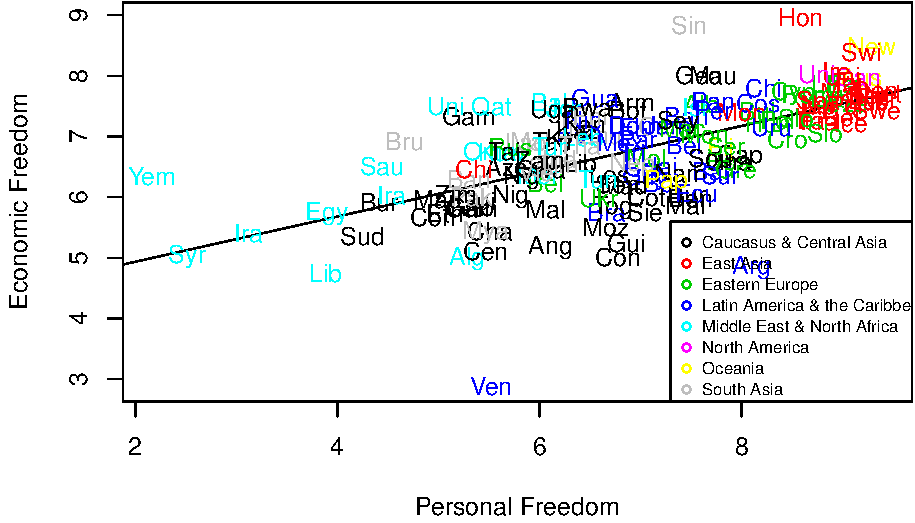
\includegraphics{final_presentation_files/figure-beamer/fig1-1.pdf}
There is a clear positive correlation between personal and economic
freedom, with a correlation of 0.6271777.

\end{frame}

\begin{frame}{Economic Freedom vs.~Rule of Law}
\protect\hypertarget{economic-freedom-vs.rule-of-law}{}

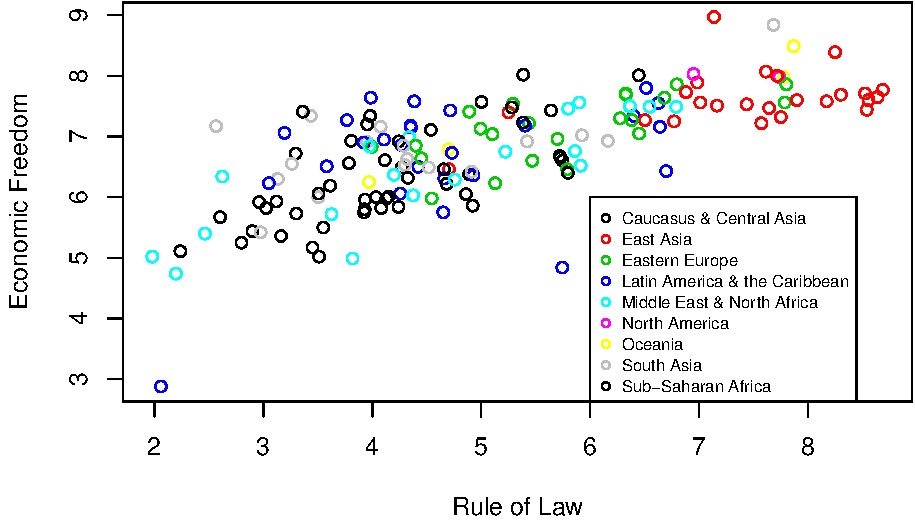
\includegraphics{final_presentation_files/figure-beamer/unnamed-chunk-3-1.pdf}

\end{frame}

\begin{frame}{Economic Freedom vs.~Security and Safety}
\protect\hypertarget{economic-freedom-vs.security-and-safety}{}

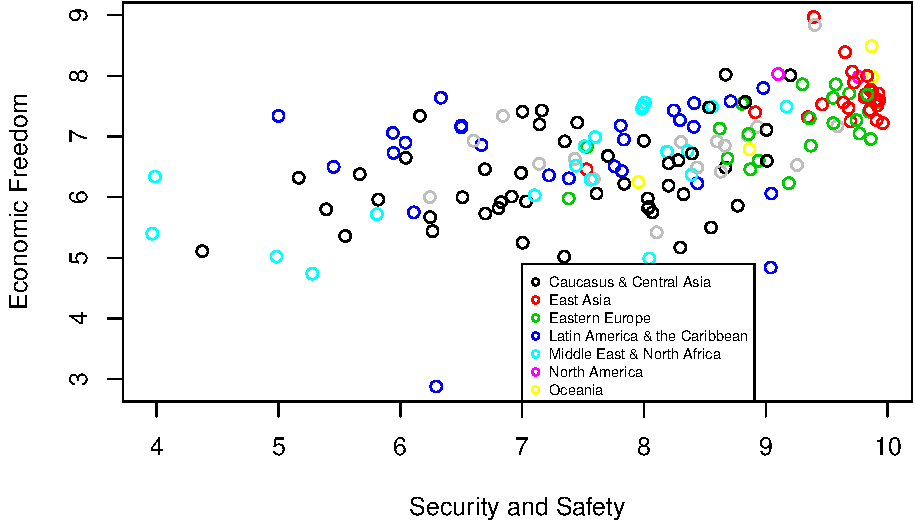
\includegraphics{final_presentation_files/figure-beamer/unnamed-chunk-4-1.pdf}

\end{frame}

\begin{frame}{Economic Freedom vs.~Movement}
\protect\hypertarget{economic-freedom-vs.movement}{}

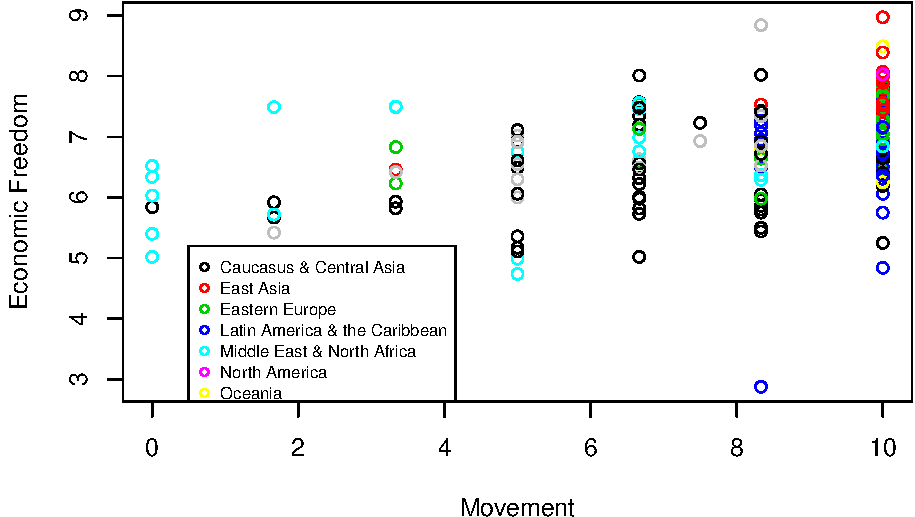
\includegraphics{final_presentation_files/figure-beamer/unnamed-chunk-5-1.pdf}

\end{frame}

\begin{frame}{Economic Freedom vs.~Religion}
\protect\hypertarget{economic-freedom-vs.religion}{}

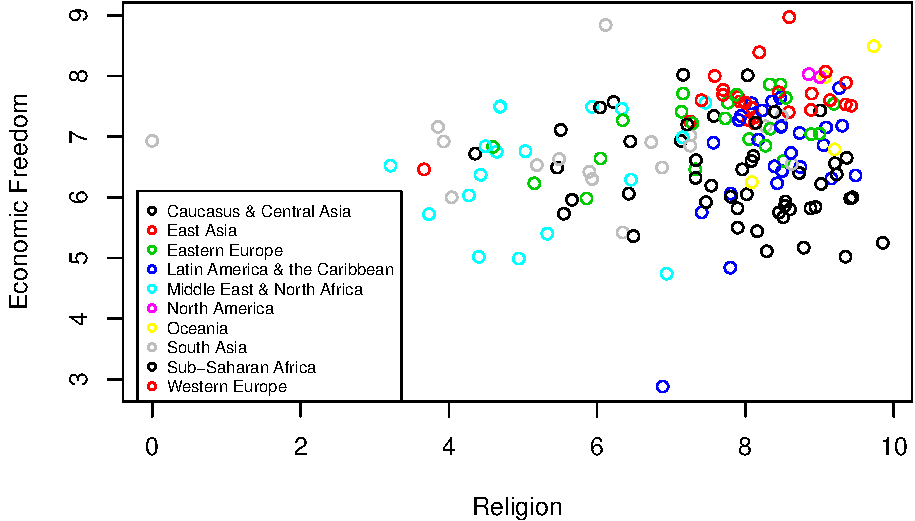
\includegraphics{final_presentation_files/figure-beamer/unnamed-chunk-6-1.pdf}

\end{frame}

\begin{frame}{Economic Freedom vs.~Association, Assembly, and Civil
Society}
\protect\hypertarget{economic-freedom-vs.association-assembly-and-civil-society}{}

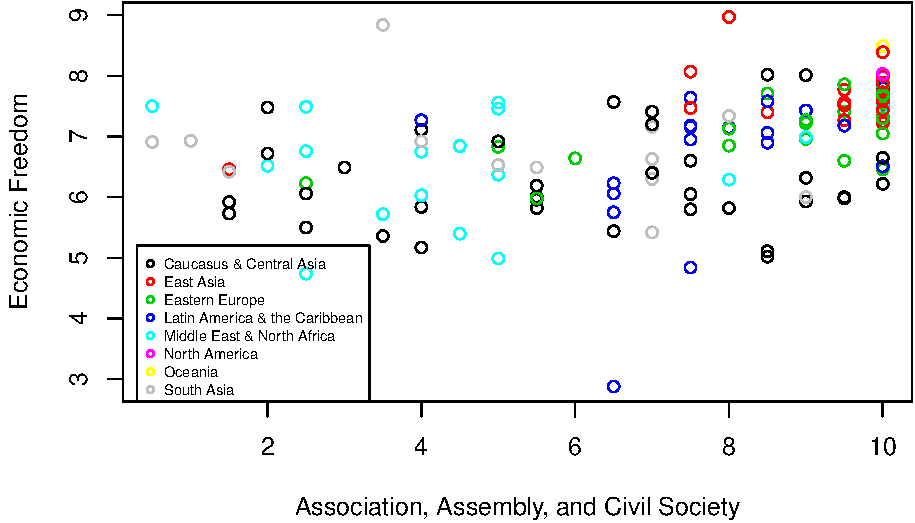
\includegraphics{final_presentation_files/figure-beamer/unnamed-chunk-7-1.pdf}

\end{frame}

\begin{frame}{Economic Freedom vs.~Expression and Information}
\protect\hypertarget{economic-freedom-vs.expression-and-information}{}

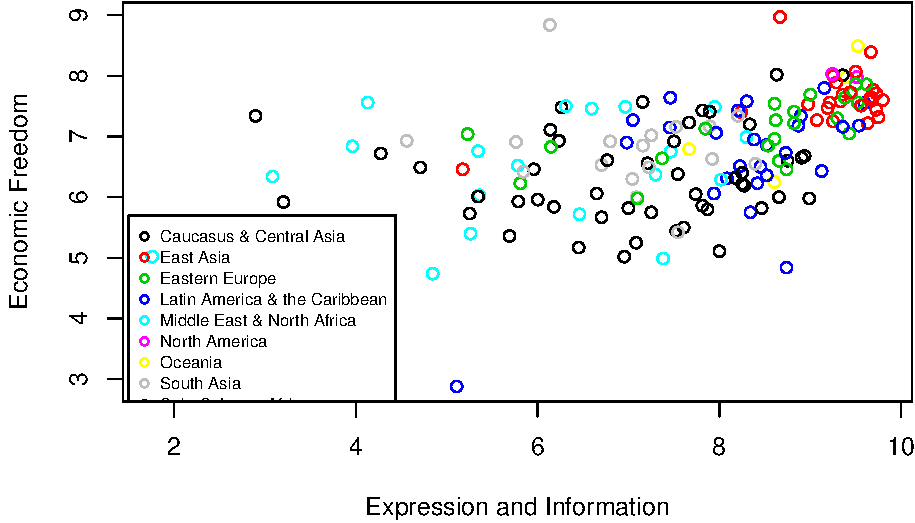
\includegraphics{final_presentation_files/figure-beamer/unnamed-chunk-8-1.pdf}

\end{frame}

\begin{frame}{Economic Freedom vs.~Identity and Relationships}
\protect\hypertarget{economic-freedom-vs.identity-and-relationships}{}

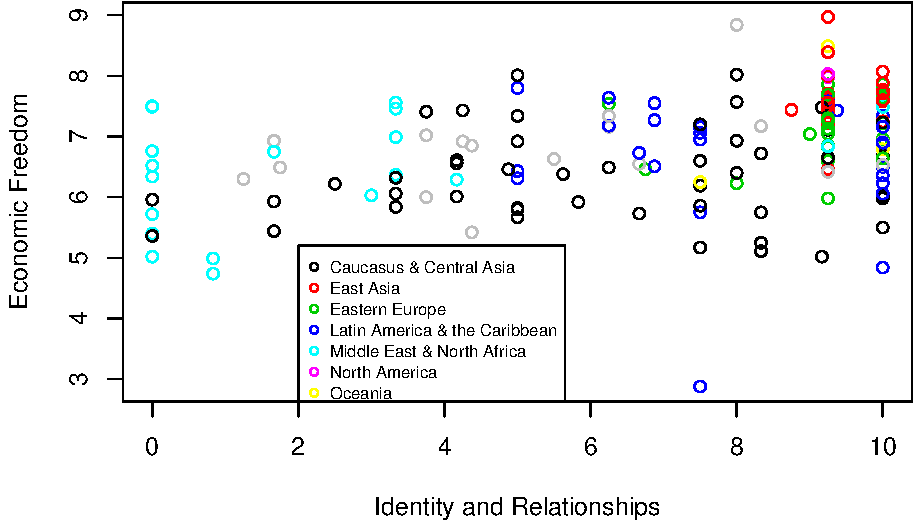
\includegraphics{final_presentation_files/figure-beamer/unnamed-chunk-9-1.pdf}

\end{frame}

\begin{frame}[fragile]{Multiple Regression of Economic Freedom and
Sub-Categories of Personal Freedom}
\protect\hypertarget{multiple-regression-of-economic-freedom-and-sub-categories-of-personal-freedom}{}

\begin{verbatim}
## 
## Call:
## lm(formula = data$economicfreedom ~ data$rol + data$religion + 
##     data$expression + data$safety + data$relationships + data$movement + 
##     data$assembly)
## 
## Residuals:
##      Min       1Q   Median       3Q      Max 
## -2.82288 -0.34787 -0.01219  0.37809  1.32904 
## 
## Coefficients:
##                     Estimate Std. Error t value Pr(>|t|)    
## (Intercept)         4.039267   0.450908   8.958 3.32e-15 ***
## data$rol            0.301251   0.051946   5.799 4.92e-08 ***
## data$religion      -0.005481   0.046958  -0.117   0.9073    
## data$expression    -0.008769   0.079106  -0.111   0.9119    
## data$safety         0.121946   0.062657   1.946   0.0538 .  
## data$relationships -0.006516   0.023991  -0.272   0.7864    
## data$movement       0.044263   0.029082   1.522   0.1305    
## data$assembly       0.005833   0.039250   0.149   0.8821    
## ---
## Signif. codes:  0 '***' 0.001 '**' 0.01 '*' 0.05 '.' 0.1 ' ' 1
## 
## Residual standard error: 0.6266 on 128 degrees of freedom
##   (26 observations deleted due to missingness)
## Multiple R-squared:  0.5607, Adjusted R-squared:  0.5367 
## F-statistic: 23.34 on 7 and 128 DF,  p-value: < 2.2e-16
\end{verbatim}

\end{frame}

\begin{frame}[fragile]{Correlation Between Rule of Law and
Sub-Categories of Personal Freedom}
\protect\hypertarget{correlation-between-rule-of-law-and-sub-categories-of-personal-freedom}{}

\begin{verbatim}
##            [,1]
## [1,] -0.3282557
## [2,]  0.9044933
## [3,]  0.5227554
## [4,]  0.6780413
## [5,]  0.6852750
\end{verbatim}

\end{frame}

\begin{frame}{Conclusion}
\protect\hypertarget{conclusion}{}

There is a significant relation between economic and personal freedom;
one can be predicted using the other. From the summary of the
regression, we were able to conclude that Rule of Law is the most
signifant in the prediction of economic freedom. Therefore, we examined
the correlation between the rule of law index and the subcategories of
economic freedom.

\end{frame}

\end{document}
